Nesse capítulo, serão apresentados os resultados obtidos utilizando o método multiescala para solução dos sistemas lineares decorrentes do operador apresentado em \ref{ch:modelagem}. Os resultados são apresentados na seguinte ordem: resultados em casos que a solução analítica é conhecida para testar o bom funcionamento do método, comparações do método multiescala como pré-condicionador e resultados do método multiescala como solver linear.



\begin{table}[]
\caption{Tabela com os casos que serão apresentados os resultados}
\centering
\begin{tabular}{ccccl}
\cline{1-4}
\multicolumn{1}{|c|}{\textbf{Nome}} & \multicolumn{1}{c|}{\textbf{Nx}} & \multicolumn{1}{c|}{\textbf{Ny}} & \multicolumn{1}{c|}{\textbf{Caso Real}} &  \\ \cline{1-4}
\multicolumn{1}{|c|}{caso A}        & \multicolumn{1}{c|}{100}         & \multicolumn{1}{c|}{100}         & \multicolumn{1}{c|}{}                   &  \\ \cline{1-4}
\multicolumn{1}{|c|}{caso B}        & \multicolumn{1}{c|}{320}         & \multicolumn{1}{c|}{320}         & \multicolumn{1}{c|}{}                   &  \\ \cline{1-4}
\multicolumn{1}{|c|}{caso C}        & \multicolumn{1}{c|}{103}         & \multicolumn{1}{c|}{56}          & \multicolumn{1}{c|}{}                   &  \\ \cline{1-4}
\multicolumn{1}{|c|}{caso D}        & \multicolumn{1}{c|}{244}            & \multicolumn{1}{c|}{71}            & \multicolumn{1}{c|}{Sim}                &  \\ \cline{1-4}
\multicolumn{1}{|c|}{caso  E}       & \multicolumn{1}{c|}{582}         & \multicolumn{1}{c|}{336}         & \multicolumn{1}{c|}{Sim}                &  \\ \cline{1-4}
\multicolumn{1}{l}{}                & \multicolumn{1}{l}{}             & \multicolumn{1}{l}{}             & \multicolumn{1}{l}{}                    &  \\
\multicolumn{1}{l}{}                & \multicolumn{1}{l}{}             & \multicolumn{1}{l}{}             & \multicolumn{1}{l}{}                    & 
\end{tabular}
\end{table}


\section{Soluções Analíticas}

Para atestar o bom resultado do método, é importante comparar com soluções que são conhecidas analiticamente. Os testes apresentados são incrementais de forma a testar que todas as opções estão funcionando corretamente.

Primeiro, são apresentados casos onde as condições de contorno são de Dirichlet Homogêneas. Esse teste é aplicado no domínio $ \Omega = [0, 2] \times [0, 2]$ com solução apresentada em \ref{eq:solucaoDirichletHomogeneo};

\begin{equation}\label{eq:solucaoDirichletHomogeneo}
u = 
\begin{bmatrix}
u_x
\\ 
u_y
\end{bmatrix}
=
\begin{bmatrix}
y(-y+2)sen(\pi x))
\\ 
x(-x+2)sen(\pi x))
\end{bmatrix}
\end{equation}É importante notar que os valores da solução na fronteira do domínio são zero. Pode-se calcular o lado direito referente dessa solução aplicando o operador do problema. Fazendo isso, o lado direito encontrado é o mostrado em \ref{eq:ldDiricheletHomogeneo}.

\begin{equation}\label{eq:ldDiricheletHomogeneo}
f(x, y) = 
\left[\begin{matrix}
\begin{split}
\frac{\pi E v x}{v^{2} - 1} \cos{\left (\pi y \right )} - \frac{\pi E v}{v^{2} - 1} \left(- x + 2\right) \cos{\left (\pi y \right )} + \frac{\pi^{2} E y}{v^{2} - 1} \left(- y + 2\right) \sin{\left (\pi x \right )} 
\\
+
\frac{E}{2 v + 2} \left(- \pi x \cos{\left (\pi y \right )} + \pi \left(- x + 2\right) \cos{\left (\pi y \right )} - 2 \sin{\left (\pi x \right )}\right)
\end{split}
\\

\frac{\pi E v y}{v^{2} - 1} \cos{\left (\pi x \right )} - \frac{\pi E v}{v^{2} - 1} \left(- y + 2\right) \cos{\left (\pi x \right )} 
\\
+ \frac{\pi^{2} E x}{v^{2} - 1} \left(- x + 2\right) \sin{\left (\pi y \right )} + \frac{E}{2 v + 2} \left(- \pi y \cos{\left (\pi x \right )} + \pi \left(- y + 2\right) \cos{\left (\pi x \right )} - 2 \sin{\left (\pi y \right )}\right)\end{matrix}\right]
\end{equation}


Assim, o problema \ref{eq:problemaDirichlet}.

\begin{equation} \label{eq:problemaDirichlet}
\begin{matrix}
\nabla \cdot  (C_{dr} : \nabla ^s u) = f(x,y)
\\ 
u_x (x, y)  =  0, \text{em } \partial \Omega
\\ 
u_y (x, y)  =  0, \text{em } \partial \Omega

\end{matrix}
\end{equation}

A figura \ref{fig:DirichletHomogeneo} apresenta a comparação entre a solução de um grid fino contra a solução do grid grosso.  

\begin{figure}[!htbp]
\label{fig:DirichletHomogeneo}
\centering
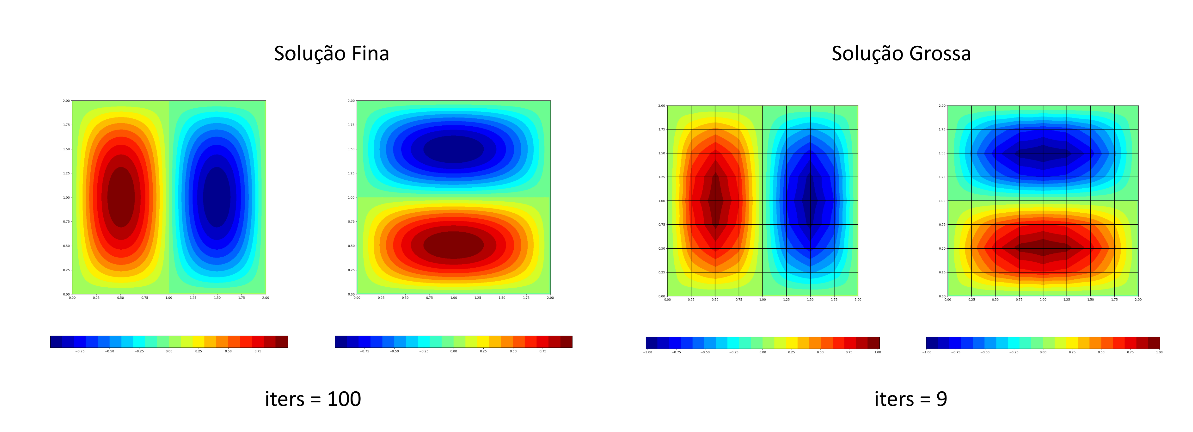
\includegraphics[width=6cm]{chap08/figs/DirichletHomogeneoTemp.png}
\caption{Comparação entre solução do grid fino e do grid grosso. }
\end{figure}


O segundo executado é utilizando a mesma solução anterior mas com domínio $\Omega = [0, 2] \times [0, 1]$, mas agora com condição de Neumann homogênea na fronteira $y=1$. Como a solução não mudou, o lado direito continua da mesma forma que o primeiro caso.

A figura \ref{fig:NeumannHomogeneo} apresenta a solução do grid fino contra a solução do grid grosso.

\begin{figure}[!htbp]
\label{fig:NeumannHomogeneo}
\centering
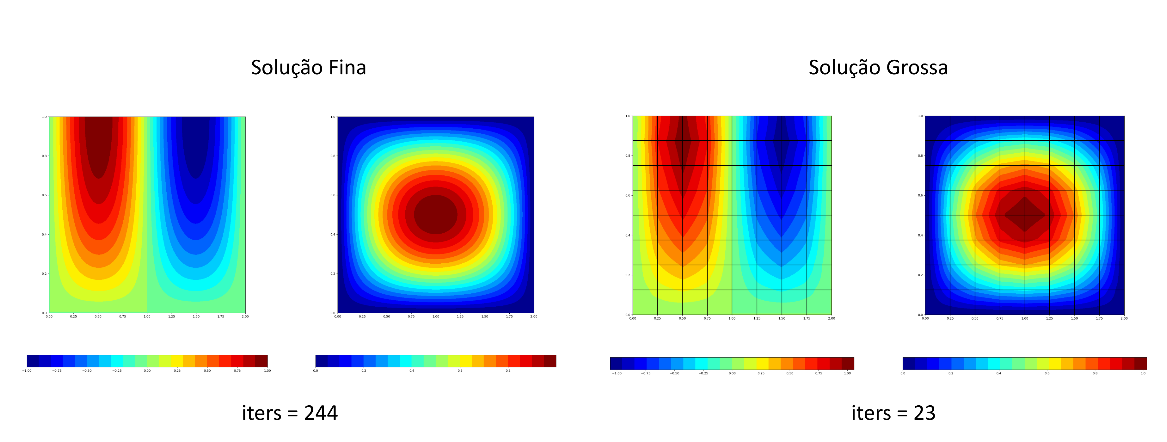
\includegraphics[width=6cm]{chap08/figs/NeumannHomogeneoTemp.png}
\caption{Comparação entre solução do grid fino e do grid grosso. }
\end{figure}



\section{Método Multiescala como pré-condicionador}

\subsection{Comparação entre pré-condicionadores aditivos e multiplicativos}

O trabalho \cite{casteletto} apresenta a utilização do pré-condicionador multiescala ($M_{ms}$) em conjunto com o um pré-condicionador ($M_h$) no grid fino  de forma multiplicativa. Essa combinação visa reduzir os erros de alta frequência através do $M_h$ enquanto os erros de baixa frequencia são eliminados pelo pré-condicionador multiescala. Esse acoplamento tem a desvantagem de precisar de uma multiplicação matriz vetor além da aplicação dos pré-condicionadores utilização desse tipo de acoplamento pode trazer ganhos na redução do tempo de simulação do sistema. 

Foram utilizados o caso A e caso B para essa comparação. As tabelas \ref{tab:precondcasoAcomp} e \ref{tab:precondcasoBcomp} mostram a quantidade de iterações feita pelos pré-condicionadores aplicados a solução do sistema desses dois reservatórios. 



\begin{table}[]\label{tab:precondcasoAcomp}
\caption{Comparação de pré-condicionador aditivo contra multiplicativo para caso A}
\centering
\begin{tabular}{|c|c|c|c|c|}
\hline
\multirow{2}{*}{\begin{tabular}[c]{@{}c@{}}Precondicionador\\ Elemento Grosso\end{tabular}} & \multicolumn{2}{c|}{$\preconmult$} & \multicolumn{2}{c|}{$\preconadd$} \\ \cline{2-5} 
                                                                                             & Iterações      & Resíduo           & Iterações      & Resíduo          \\ \hline
2x2                                                                                        & 6              & 2.000986e-07      & 9              & 9.330103e-07     \\ \hline
5x5                                                                                          & 11             & 7.823222e-07      & 15             & 5.421610e-07     \\ \hline
10x10                                                                                          & 20             & 6.668921e-07      & 24             & 8.444513e-07     \\ \hline
\end{tabular}
\end{table}


\begin{table}[]\label{tab:precondcasoBcomp}
\caption{Comparação de pré-condicionador aditivo contra multiplicativo para caso B}
\centering
\begin{tabular}{|c|c|c|c|c|}
\hline
\multirow{2}{*}{\begin{tabular}[c]{@{}c@{}}Precondicionador\\ Elemento grosso\end{tabular}} & \multicolumn{2}{c|}{$\preconmult$} & \multicolumn{2}{c|}{$\preconadd$} \\ \cline{2-5} 
                                                                                             & Iterações      & Resíduo           & Iterações      & Resíduo          \\ \hline
32x32                                                                                        & 66             & 9.892304e-07      & 72             & 9.232924e-07     \\ \hline
64x64                                                                                        & 115            & 8.366432e-07      & 115            & 8.845719e-07     \\ \hline
80x80                                                                                        & 126            & 8.811373e-07      & 124            & 9.607785e-07     \\ \hline
\end{tabular}
\end{table}




\subsection{Comparação com Multigrid}

Nessa seção, são apresentadas comparações entre o pré-condicionador multiescala e o solver multigrid. Para esse comparação foi utilizado o solver multigrid Pyamg descrito e implementado em \cite{OlSc2018}. Dado a grande quantidade de parâmetros necessários para a configuração dos solver multigrid como: a quantidade de níveis devem ser utilizados, quantidade de relaxações em cada nível, qual o tipo de relaxação será utilizada, dentre outras variáveis, foi utilizado o script solver\_diagnotics.py disponibilizado pela equipe do Pyamg no repositório ( https://github.com/pyamg/pyamg-examples ). Esse script testa sessenta diferentes configurações de solver multigrid e seleciona aquele mais eficiente para o problema proposto.

Os resultados para cada uma das matrizes utilizando mostrou que os solver selecionados como parâmetros: no máximo 15 níveis multigrid, como relaxação utilizavam o "Block Gauss Seidel Sweep" e ciclos V. Sobre a relaxação, o Gauss Seidel Sweep é composta pela aplicação da versão é aplicada nos dois sentidos, atualizando primeiramente o valor  $x_1$  do vetor e depois uma iteração atualizando primeiro o valor  $x_n$. Outra escolha comum para todos os casos, foi a utilização do multigrid como pré-condicionador para o gradiente conjugado.


A figura \ref{fig:reservatorio100x100_1} apresenta o tempo de solução do sistema utilizando o método multiescala e multigrid (Pyamg) como precondicionador para o gradiente conjugado. São apresentados o resíduo ao longo das iterações, o tempo de execução do solver, a quantidade de iterações do solver linear e o tempo da iteração.

\begin{figure}[!htbp]
\label{fig:reservatorio100x100_1}
\centering
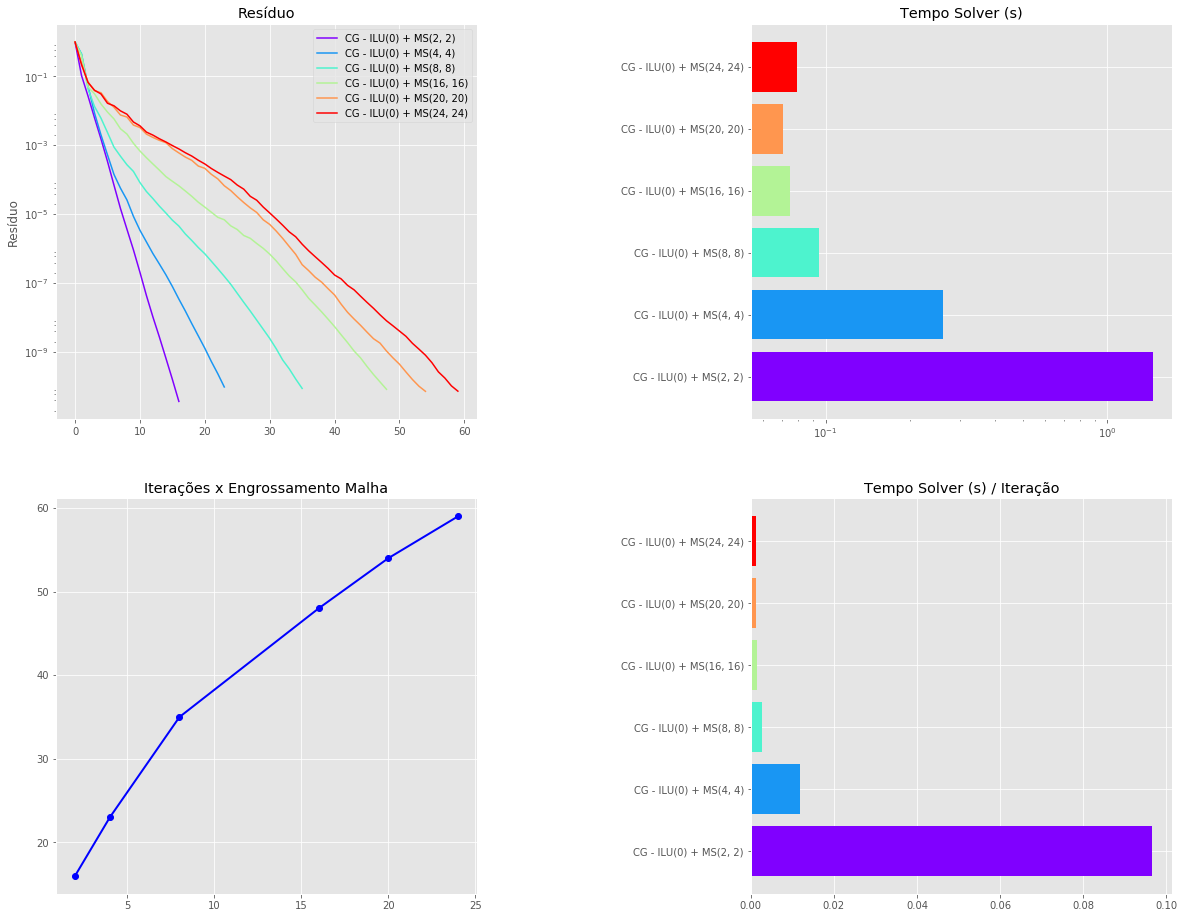
\includegraphics[width=\textwidth]{chap08/figs/reservatorio100x100_1.png}
\caption{Resultados para caso A. Histórico do resíduo relativo ao longo das iterações, tempo do solver em segundos, número de iterações em função do fator de engrossamento da malha e tempo do solver por iteração. }
\end{figure}

Um primeiro ponto a se observar é o aumento do número de iterações a cada vez que se aumenta o fator de engrossamento da malha. Isso ocorre pois a solução do problema grosso se torna cada vez mais distante da solução  original quanto mais a malha perde resolução. Porém, quanto mais grossa a malha, mais rapidamente o sistema linear é resolvido, portanto, existe uma solução de compromisso entre o engrossamento da malha e a quantidade de iterações que serão necessárias para resolver o sistema linear. No caso A, a solução de menor tempo é quando o nível grosso é construído ao se montar elementos grossos utilizando 8x8 elementos finos. 

Na figura \ref{fig:reservatorio100x100_2} é apresentado agora a comparação da solução do sistema utilizando o melhor método multiescala com o gradiente conjugado utilizando como precondicionador o ILU(0), ILU(1) e solver multigrid Pyamg. Pode-se notar que apesar da redução de iterações dos método multiescala e do método multigrid, os pré-condicionadores ILU(0) e ILU(1) são mais eficientes na resolução do sistema. 


\begin{figure}[!htbp]
\label{fig:reservatorio100x100_2}
\centering
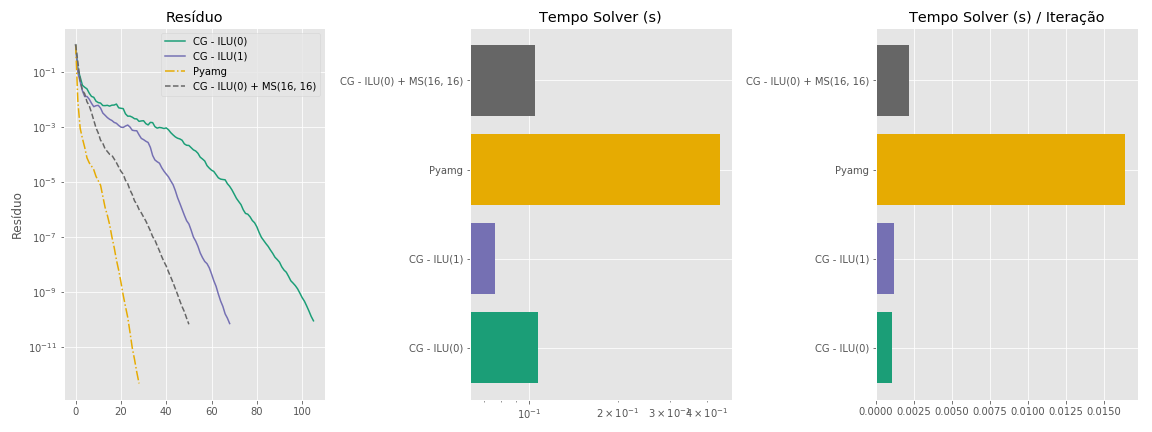
\includegraphics[width=\textwidth]{chap08/figs/reservatorio100x100_2.png}
\caption{Resultados para caso A. Histórico do resíduo relativo ao longo das iterações, tempo do solver em segundos, número de iterações em função do fator de engrossamento da malha e tempo do solver por iteração. }
\end{figure}


As figuras \ref{fig:reservatorio320x320_1} e \ref{fig:reservatorio320x320_2} apresentam os mesmos resultados para o caso B. Nesse caso, o engrossamento multiescala de 20x20 é o que resolve o solver em menor tempo, conseguindo inclusive superar o tempo de solução com o solver pré-condicionador ILU(1).


\begin{figure}[!htbp]
\label{fig:reservatorio320x320_1}
\centering
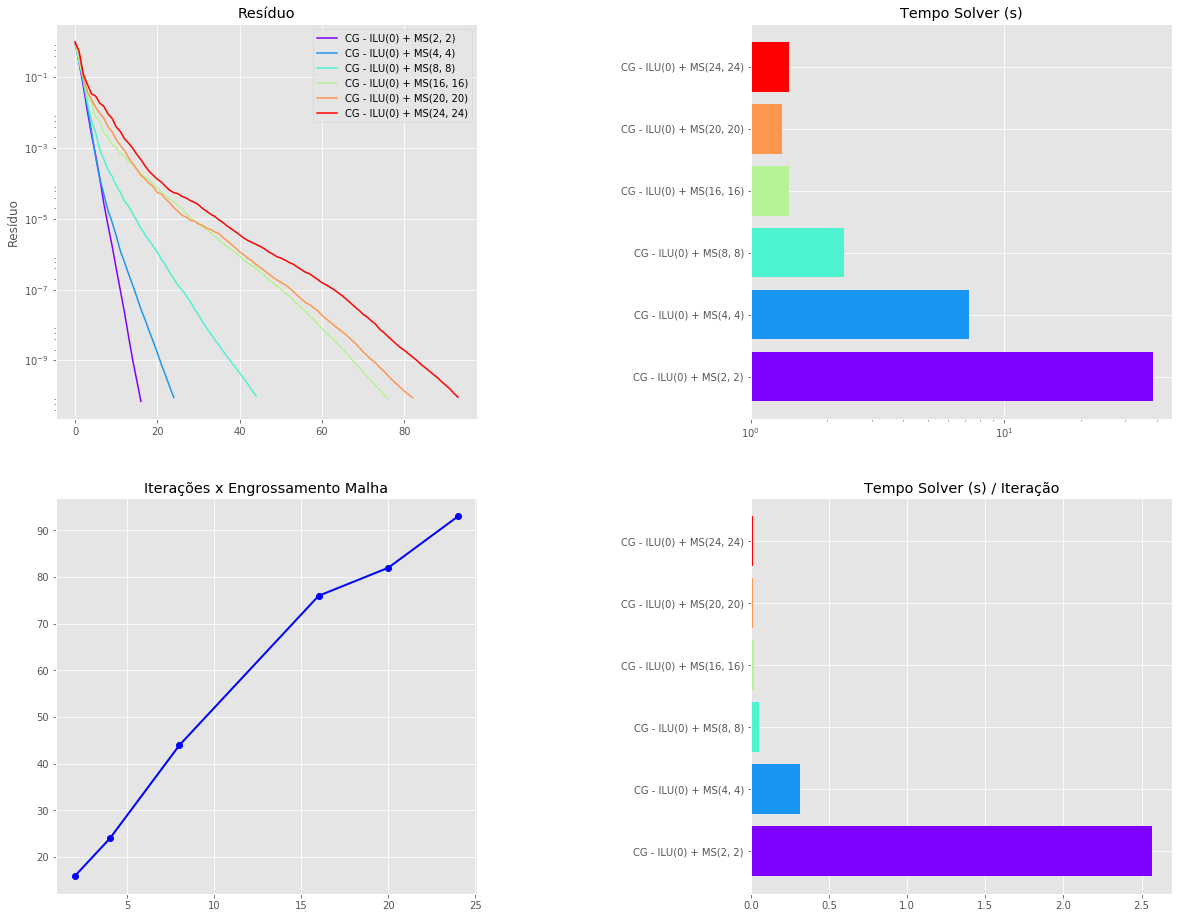
\includegraphics[width=\textwidth]{chap08/figs/reservatorio320x320_1.png}
\caption{Resultados para caso B. Histórico do resíduo relativo ao longo das iterações, tempo do solver em segundos, número de iterações em função do fator de engrossamento da malha e tempo do solver por iteração. }
\end{figure}


\begin{figure}[!htbp]
\label{fig:reservatorio320x320_2}
\centering
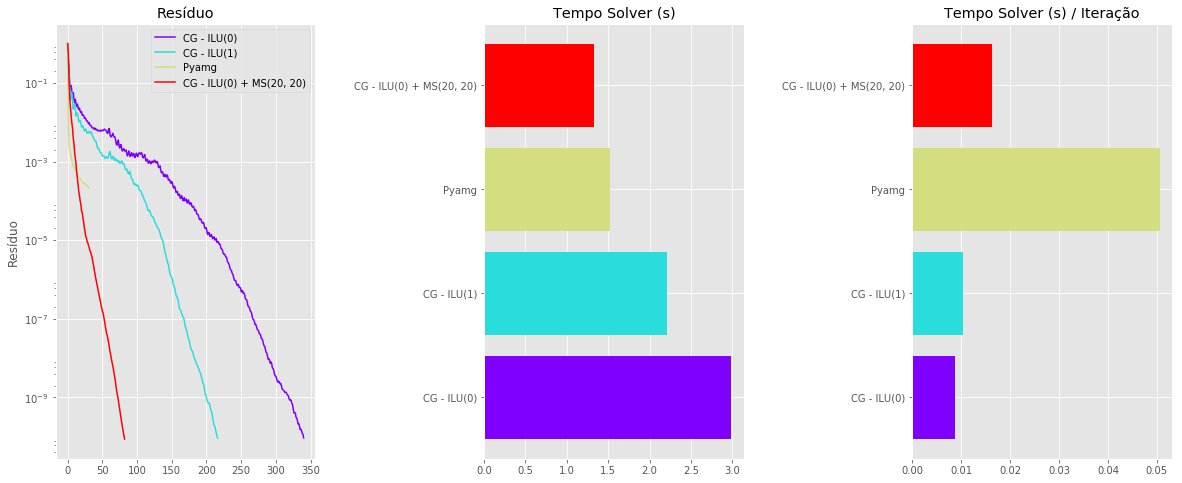
\includegraphics[width=\textwidth]{chap08/figs/reservatorio320x320_2.png}
\caption{Resultados para caso B. Histórico do resíduo relativo ao longo das iterações, tempo do solver em segundos, número de iterações em função do fator de engrossamento da malha e tempo do solver por iteração. }
\end{figure}


A seguir, as figuras \ref{fig:casoC_2}, \ref{fig:casoD_2} e \ref{fig:casoE_2} apresentam os resultados para os casos C, D e E. Em todos os gráficos é mostrado apenas o pré-condicionador multiescala que obteve o melhor desempenho entre os fatores de engrossamento de 2x2, 4x4, 8x8, 16x16, 32x32.


% \begin{figure}[!htbp]
% \label{fig:casoC_1}
% \centering
% 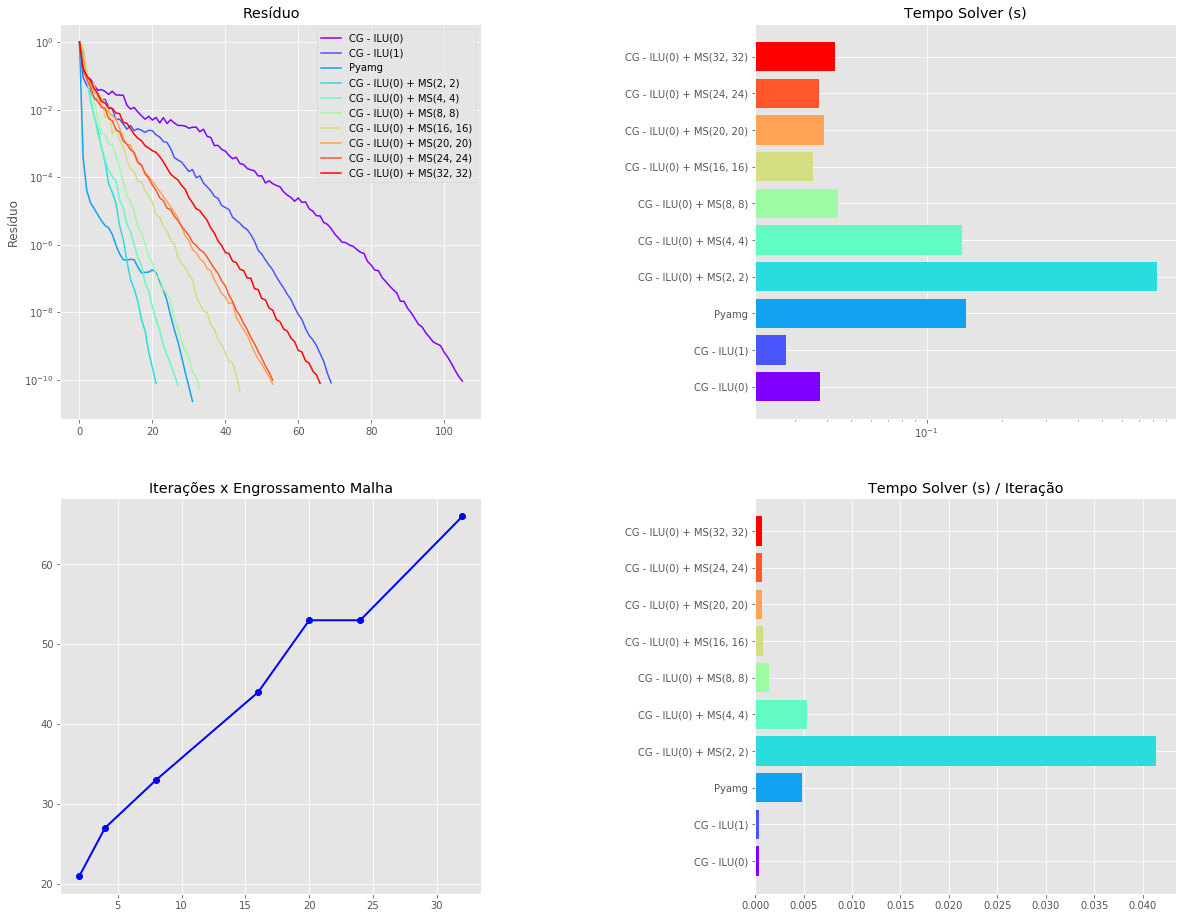
\includegraphics[width=\textwidth]{chap08/figs/casoC_1.png}
% \caption{Resultados para caso C. Histórico do resíduo relativo ao longo das iterações, tempo do solver em segundos, número de iterações em função do fator de engrossamento da malha e tempo do solver por iteração. }
% \end{figure}

\begin{figure}[!htbp]
\label{fig:casoC_2}
\centering
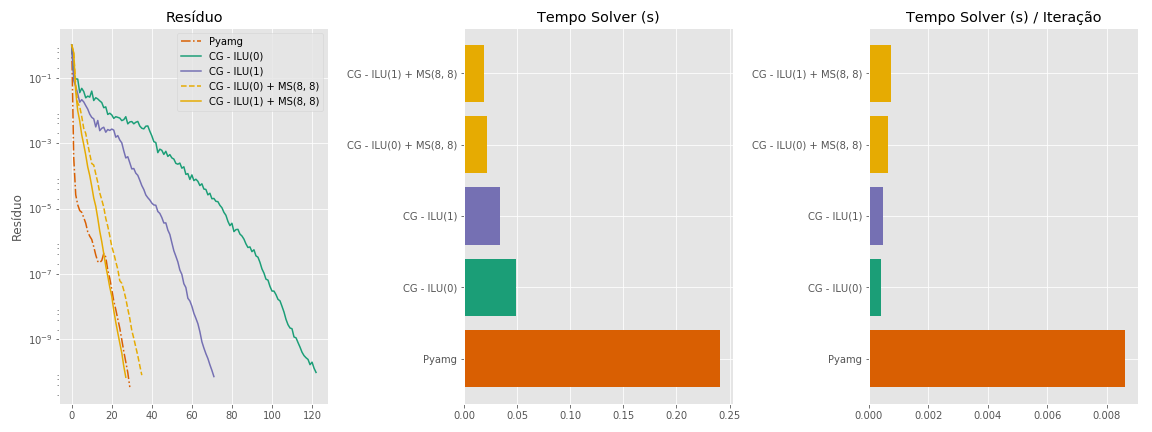
\includegraphics[width=\textwidth]{chap08/figs/casoC_2.png}
\caption{Comparação entre multiescala, multigrid e pré-condicionador ILU para o caso C. Histórico do resíduo relativo ao longo das iterações, tempo do solver em segundos e tempo do solver por iteração. }
\end{figure}



% \begin{figure}[!htbp]
% \label{fig:casoD_1}
% \centering
% 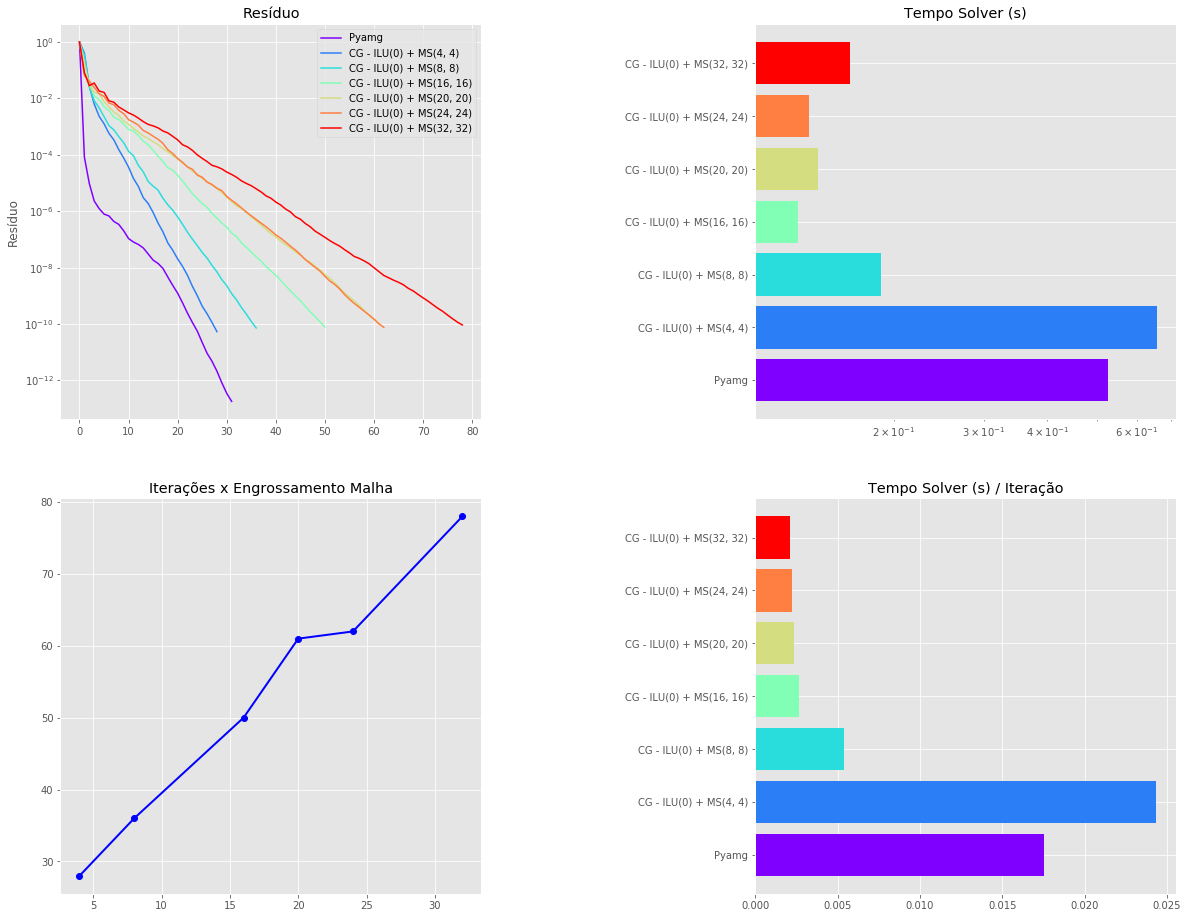
\includegraphics[width=\textwidth]{chap08/figs/casoD_1.png}
% \caption{Resultados para caso D. Histórico do resíduo relativo ao longo das iterações, tempo do solver em segundos, número de iterações em função do fator de engrossamento da malha e tempo do solver por iteração. }
% \end{figure}

\begin{figure}[!htbp]
    \label{fig:casoD_2}
    \centering
    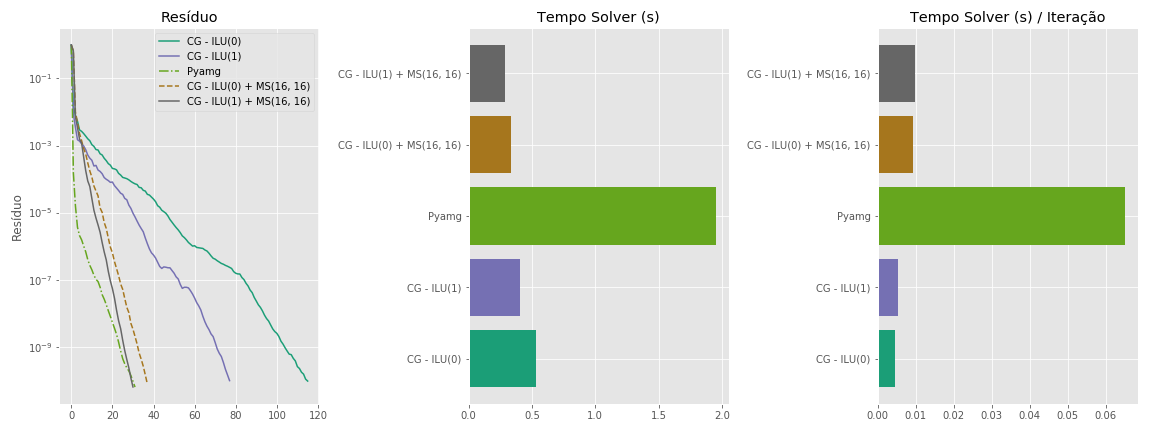
\includegraphics[width=\textwidth]{chap08/figs/casoD_2.png}
    \caption{Comparação entre multiescala, multigrid e pré-condicionador ILU para o caso D. Histórico do resíduo relativo ao longo das iterações, tempo do solver em segundos e tempo do solver por iteração. }
    \end{figure}
    
    % \begin{figure}[!htbp]
    % \label{fig:casoE_1}
    % \centering
    % 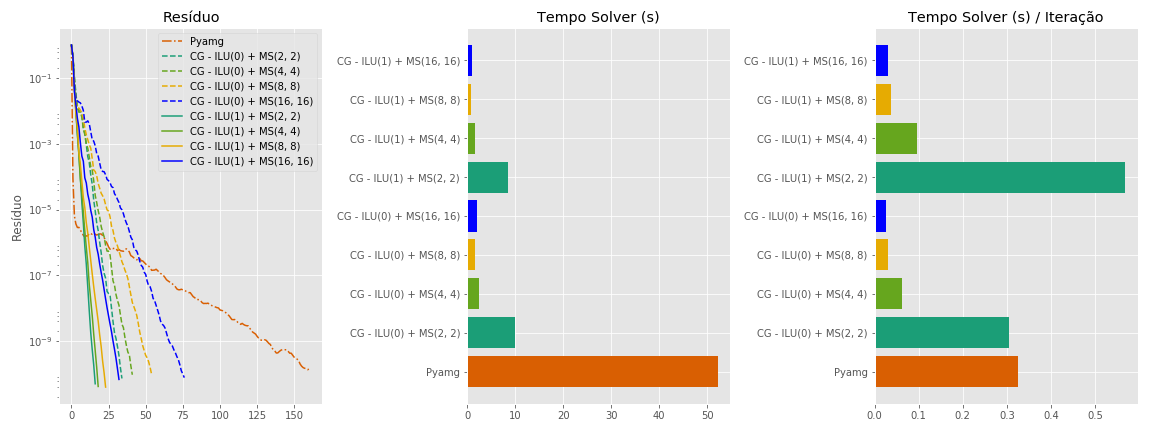
\includegraphics[width=\textwidth]{chap08/figs/casoE_1.png}
    % \caption{Resultados para caso E. Histórico do resíduo relativo ao longo das iterações, tempo do solver em segundos, número de iterações em função do fator de engrossamento da malha e tempo do solver por iteração. }
    % \end{figure}
    
    \begin{figure}[!htbp]
    \label{fig:casoE_2}
    \centering
    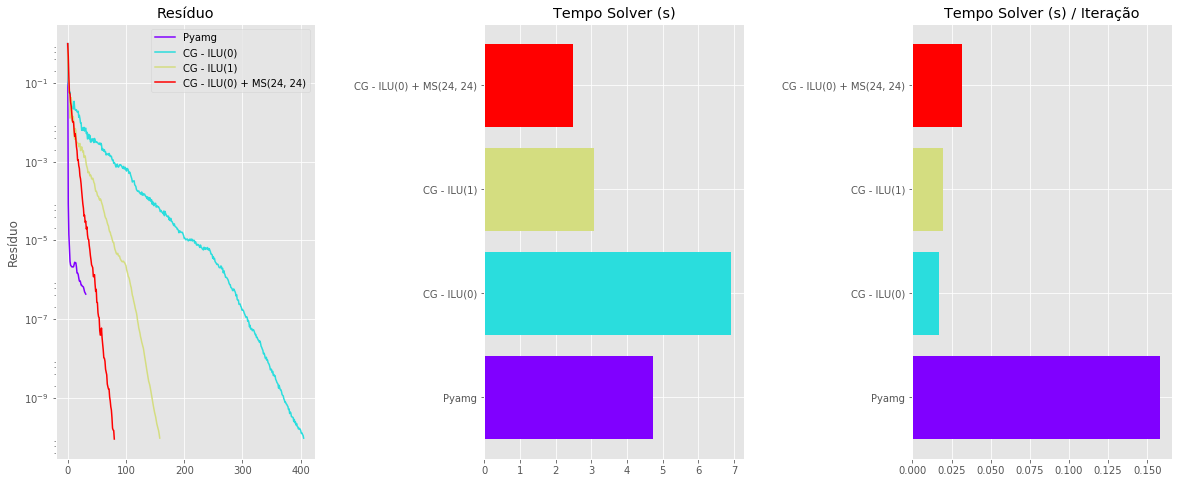
\includegraphics[width=\textwidth]{chap08/figs/casoE_2.png}
    \caption{Comparação entre multiescala, multigrid e pré-condicionador ILU para o caso D. Histórico do resíduo relativo ao longo das iterações, tempo do solver em segundos e tempo do solver por iteração. }
    \end{figure}
